\chapter{Theoretische Grundlagen}


\section{Sensoren} \label{sensoren:section}

    \subsection{Magnetometer} \label{magnetometer:subsection}

    Bei Magnetometern handelt es sich um Sensoren, die das Magnetfeld im Umfeld des Sensors messen können.
    Diese können sowohl in der Luft, als auch auf dem Boden eingesetzt werden.
    Meistens werden für diese Messungen Hall Sensoren oder Induktivitäts-Sensoren verwendet.
    Die Sensoren sind in der Lage, das Magnetfeld in drei Dimensionen zu messen und darzustellen.

    Die Messung des Magnetfeldes erfolgt dabei in der Regel über einen Halbleiter, der durch das Magnetfeld beeinflusst wird.
    und einer Elektronik, die das Signal aufbereitet und ausgibt.
    Magnetometer können jedoch nur die Richtung des Magnetfeldes messen, jedoch nicht die Stärke des Magnetfeldes.
    Magnetometer werden verwendet um die Ausrichtung von Geräten in bestimmten Koordinatensystemen zu bestimmen.
    Sie können für diese Ausrichtungsbestimmung auch in der Luft verwendet werden. 

    \subsection{Kamera} \label{kamera:section}

        \subsubsection{Bild Kamera} \label{bild_kamera:subsubsection}

        \subsubsection{Infrarot Kamera} \label{infrarot_kamera:subsubsection}

    \subsection{Abstandssensoren} \label{abstandssensoren:subsection}

\section{ROS - Robot Operating System} \label{ros:section}
\ac{ROS} ist eine Open-Source-Plattform, die speziell für die Entwicklung von Robotersoftware entwickelt wurde. Es bietet eine Reihe von Bibliotheken, Tools und Frameworks, die es Entwicklern ermöglichen, komplexe Robotikanwendungen zu erstellen und zu betreiben. \ac{ROS} wurde von Willow Garage entwickelt und ist heute ein weit verbreitetes Framework in der Robotik-Community.

\ac{ROS} besteht aus verschiedenen Modulen, die es ermöglichen, Roboterhard-  und software zu abstrahieren und zu standardisieren. Die Plattform bietet eine Vielzahl von Werkzeugen für die Entwicklung von Robotik-Software, einschließlich Visualisierungstools, Datenverarbeitungs- und Analysetools sowie eine umfassende Dokumentation.

\ac{ROS} ist so konzipiert, dass es auf einer Vielzahl von Betriebssystemen und Hardwarearchitekturen laufen kann und bietet Unterstützung für eine breite Palette von Robotern und Sensoren. Es ist auch bekannt für seine Fähigkeit zur Zusammenarbeit zwischen verschiedenen Robotern, die miteinander kommunizieren und Aufgaben gemeinsam erledigen können.

Dank seiner leistungsstarken Funktionen und Flexibilität ist \ac{ROS} zu einem der wichtigsten Frameworks für die Robotik-Entwicklung geworden und wird in vielen Anwendungen eingesetzt, von industriellen Robotern bis hin zu autonomen Fahrzeugen.

    \subsection{Nodes} \label{nodes:subsection}
    In \ac{ROS} werden Funktionen und Prozesse durch sogenannte Nodes realisiert. Eine Node ist eine ausführbare Einheit, die in einem \ac{ROS}-System arbeitet und über eine eindeutige Identifikation verfügt. Jede Node hat eine spezifische Aufgabe, wie beispielsweise das Sammeln von Sensordaten, die Ausführung einer spezifischen Berechnung oder das Steuern eines Aktors.

    Nodes können miteinander kommunizieren, indem sie Nachrichten senden und empfangen. Nachrichten sind definierte Datenstrukturen, die Informationen zwischen Nodes transportieren. Nodes können auch Services anbieten oder anfordern, um eine bestimmte Aktion auszuführen.

    Eine wichtige Funktion von Nodes ist ihre Fähigkeit zur Verteilung. In \ac{ROS} können Nodes auf verschiedenen Hosts oder in verschiedenen Prozessen ausgeführt werden. Dadurch können komplexe \ac{ROS}-Systeme erstellt werden, die aus vielen miteinander verbundenen Nodes bestehen.

    Nodes können auch in einer \ac{ROS}-Graphenstruktur organisiert werden. Diese Struktur zeigt die Abhängigkeiten zwischen Nodes und die Art der Kommunikation zwischen ihnen an. Die \ac{ROS}-Graphenstruktur kann mit Werkzeugen wie rqt\_graph visualisiert werden, um eine bessere Übersicht über das System zu erhalten.

    Die Verwendung von Nodes in \ac{ROS} ermöglicht eine hohe Flexibilität und Modularität bei der Entwicklung von Robotik-Anwendungen. Entwickler können einzelne Nodes erstellen, testen und optimieren, bevor sie sie in einem größeren System einsetzen. Darüber hinaus können Nodes wiederverwendet werden, um ähnliche Funktionen in verschiedenen Anwendungen auszuführen.

    Insgesamt sind Nodes eine zentrale Komponente von \ac{ROS} und ermöglichen es Entwicklern, komplexe Roboteranwendungen mit einer hohen Flexibilität und Modularität zu erstellen.

    \subsection{Topics} \label{topics:subsection}
    In \ac{ROS} werden Daten zwischen Nodes durch sogenannte Topics ausgetauscht. Ein Topic ist eine benannte Kommunikationsleitung, über die Nodes Nachrichten senden und empfangen können. Topics ermöglichen die einfache und flexible Kommunikation zwischen Nodes, ohne dass die Nodes über die genaue Identität des Empfängers Bescheid wissen müssen.

    Ein Topic hat einen bestimmten Datentyp, der definiert, welche Art von Daten zwischen Nodes ausgetauscht werden können. Es können beispielsweise Sensordaten wie Bilder oder Entfernungsmessungen, oder Steuerbefehle für Aktoren wie Motoren oder Greifer übertragen werden.

    Nodes können sich auf ein Topic abonnieren, um die Nachrichten, die auf diesem Topic veröffentlicht werden, zu empfangen. Jedes Mal, wenn eine Nachricht auf einem Topic veröffentlicht wird, wird sie an alle Nodes weitergeleitet, die auf dieses Topic abonniert sind.

    Topics können auch von Nodes veröffentlicht werden, um Nachrichten an andere Nodes zu senden. Eine Node, die ein Topic veröffentlicht, wird als Publisher bezeichnet. Der Publisher kann regelmäßig Nachrichten auf einem Topic veröffentlichen, um andere Nodes über Änderungen in der Umgebung oder im System zu informieren.

    Die Verwendung von Topics in \ac{ROS} ermöglicht eine einfache und flexible Kommunikation zwischen Nodes, was besonders in komplexen Systemen von Vorteil ist. Nodes können sich auf mehrere Topics abonnieren und Nachrichten an mehrere Topics veröffentlichen, was eine effektive und modulare Datenverarbeitung ermöglicht. Zudem können Topics auf mehreren Hosts oder in verschiedenen Prozessen ausgeführt werden, was eine Skalierung des \ac{ROS}-Systems ermöglicht.

    Insgesamt sind Topics eine wichtige Komponente von \ac{ROS} und ermöglichen es Entwicklern, eine einfache und effektive Kommunikation zwischen Nodes in Robotik-Anwendungen zu realisieren.

    \subsection{Publish and Subscripe Pattern} \label{publish_and_subscripe_pattern:subsection}
    Das Publish-Subscribe-Pattern ist ein grundlegendes Muster der \ac{ROS}-Kommunikation und ermöglicht eine effektive und modulare Datenverarbeitung in verteilten Systemen.

    Beim Publish-Subscribe-Pattern senden Nodes, die Informationen über eine bestimmte Ressource verarbeiten, die Informationen an ein Topic, das als Vermittler dient. Nodes, die an den Informationen interessiert sind, abonnieren das Topic und erhalten alle zukünftigen Nachrichten, die von Nodes veröffentlicht werden, die mit dem Topic verbunden sind.

    Dieses Muster hat mehrere Vorteile. Zum einen ermöglicht es eine flexible Architektur, in der Nodes unabhängig voneinander arbeiten und sich auf das Abonnieren und Veröffentlichen von Topics konzentrieren können, ohne die genaue Identität des Empfängers oder Senders zu kennen. Zum anderen ermöglicht es eine effektive Datenverarbeitung, da mehrere Nodes dieselben Informationen von einem Publisher erhalten können.

    Ein weiterer Vorteil des Publish-Subscribe-Patterns ist, dass es eine einfache Möglichkeit bietet, den Zustand von Ressourcen zu überwachen oder auf Änderungen in Echtzeit zu reagieren. So kann beispielsweise eine Node, die eine Kamera überwacht, die Bilder auf einem Topic veröffentlichen. Andere Nodes, die an der Verarbeitung dieser Bilder beteiligt sind, können sich auf das Topic abonnieren und die Informationen in Echtzeit verarbeiten.

    Das Publish-Subscribe-Pattern ist ein grundlegendes Konzept in \ac{ROS} und wird in der Regel für die Kommunikation zwischen Nodes verwendet. Es ermöglicht eine effektive und modulare Datenverarbeitung in verteilten Systemen und ist ein wesentlicher Bestandteil von \ac{ROS}, um komplexe Robotik-Anwendungen zu realisieren.

    \subsection{Objekterkennung} \label{objekterkennung:subsection}
    In \ac{ROS} gibt es verschiedene Methoden zur Objekterkennung, die in Robotik-Anwendungen eingesetzt werden können. Die Objekterkennung ist ein wichtiger Schritt in der automatisierten Wahrnehmung von Robotern, da sie es ihnen ermöglicht, ihre Umgebung zu verstehen und darauf zu reagieren.

    Eine häufig verwendete Methode zur Objekterkennung in \ac{ROS} ist die Verwendung von 3D-Sensoren wie Lidar oder Kinect. Diese Sensoren erfassen Daten über die Umgebung des Roboters und können dabei helfen, Objekte zu identifizieren und ihre Position und Orientierung im Raum zu bestimmen.

    Eine weitere Methode zur Objekterkennung in \ac{ROS} ist die Verwendung von Bildverarbeitungs-Algorithmen. Dabei können beispielsweise Farb- oder Formmerkmale verwendet werden, um Objekte in Bildern zu erkennen und ihre Position und Ausrichtung zu bestimmen.

    Eine weiterentwickelte Methode zur Objekterkennung in \ac{ROS} ist die Verwendung von Deep-Learning-Methoden wie Convolutional Neural Networks (CNNs). Dabei werden CNNs trainiert, um Objekte in Bildern oder Punktwolken zu erkennen und zu klassifizieren. Diese Methode erfordert jedoch ein umfangreiches Training und eine hohe Rechenleistung, um in Echtzeit ausgeführt zu werden.

    Die Objekterkennung ist ein wichtiger Schritt in der automatisierten Wahrnehmung von Robotern, da sie es ihnen ermöglicht, ihre Umgebung zu verstehen und darauf zu reagieren. \ac{ROS} bietet verschiedene Methoden zur Objekterkennung, die in Robotik-Anwendungen eingesetzt werden können. Die Wahl der richtigen Methode hängt von den Anforderungen der Anwendung ab und erfordert oft eine sorgfältige Abwägung zwischen Genauigkeit, Geschwindigkeit und Komplexität.

    \subsection{QR-Codes} \label{qr-codes:subsection}
    \ac{ROS} bietet verschiedene Möglichkeiten zur Erkennung von QR-Codes in Robotik-Anwendungen. QR-Codes sind zweidimensionale Barcodes, die Informationen wie URLs, Texte oder andere Daten enthalten können. Die Erkennung von QR-Codes kann in \ac{ROS}-basierten Anwendungen genutzt werden, um Informationen zu lesen, Roboter zu navigieren oder um eine Interaktion mit der Umgebung zu ermöglichen.

    Es gibt verschiedene \ac{ROS}-Pakete, die die QR-Code-Erkennung erleichtern. Ein Beispiel ist das "zbar\_ros" Paket, das ein Wrapper für die Open-Source-ZBar-Bibliothek ist, die QR-Codes und andere Barcodes erkennt. Das zbar\_ros-Paket ermöglicht es, den Inhalt von QR-Codes aus dem Kamerabild zu extrahieren und als \ac{ROS}-Topic zu veröffentlichen, der von anderen Nodes abonniert werden kann. Das Paket bietet auch Optionen zur Konfiguration der QR-Code-Erkennung, wie beispielsweise die Festlegung der Mindestgröße des Codes oder die Einstellung der Scan-Frequenz.

    Ein weiteres \ac{ROS}-Paket, das die QR-Code-Erkennung erleichtert, ist das "ros\_qr\_detector" Paket. Dieses Paket basiert auf der OpenCV-Bibliothek und bietet eine einfache Möglichkeit, QR-Codes in \ac{ROS}-basierten Anwendungen zu erkennen. Das Paket bietet auch die Möglichkeit, QR-Codes aus der Kamerabildanzeige auszuschneiden und als separate Bilder zu speichern.

    Die Erkennung von QR-Codes in \ac{ROS}-Anwendungen kann für verschiedene Anwendungsfälle nützlich sein. Beispielsweise können QR-Codes als Marker verwendet werden

\section{Drohne/Multicopter} \label{drohne:section}
Bei der für das Projekt verwendete Drohne handelt es sich um eine Coex Clover Drohne. Dies ist eine programmierbare Drohne, die besonders für Bildungszwecke eingesetzt wird. Sie ist sowohl für den Einsatz draußen sowie auch in Gebäuden geeignet. \\

\begin{figure}[htpb]
    \centering
    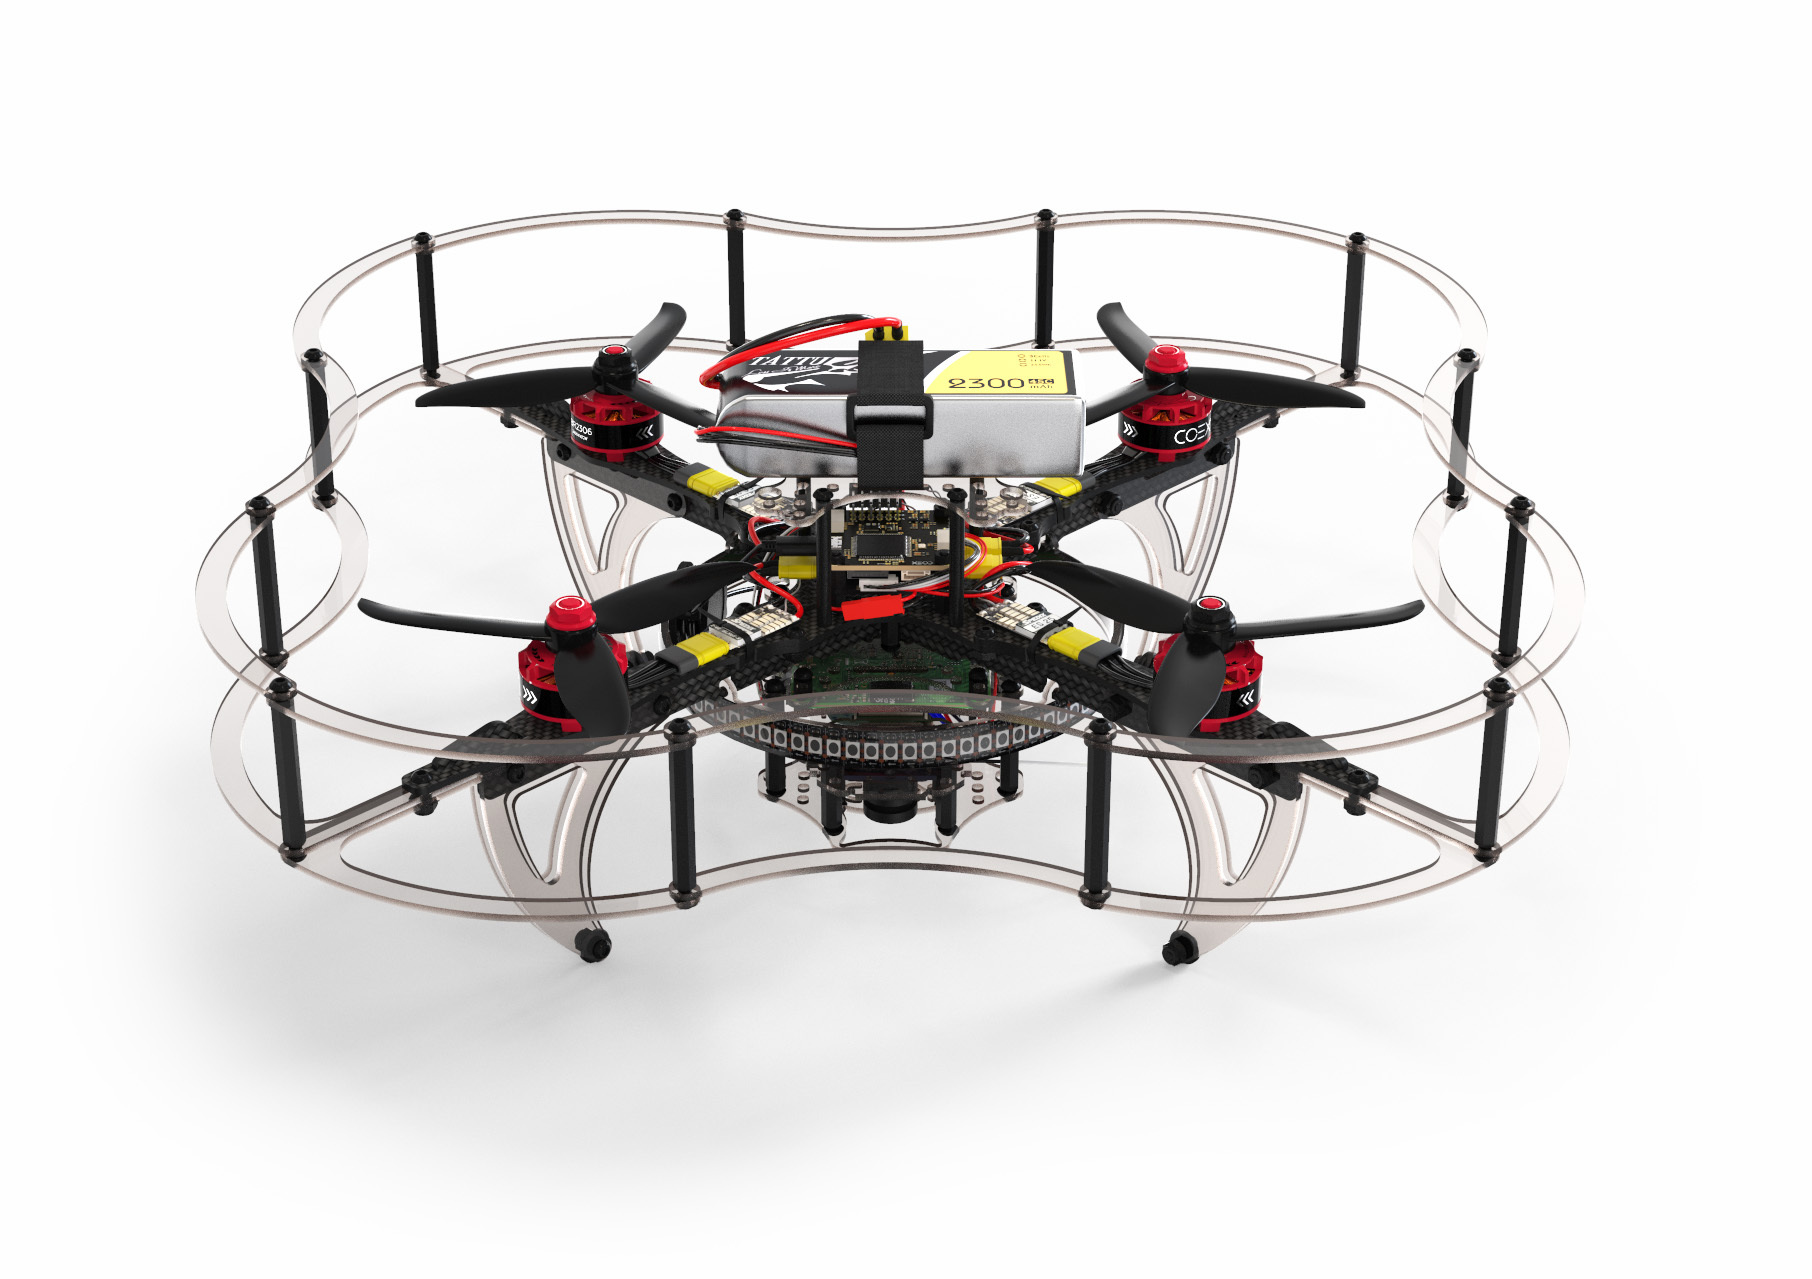
\includegraphics[width=10cm,keepaspectratio,angle=0]{images/coex_clover.jpg}
    \caption[Coex Clover Drohne]{\label{img coex_clover} Coex Clover Drohne \cite{img_coex_clover}}
\end{figure}


Zu Beginn erhält man hierbei einen Bausatz, welcher dann zu einem Quadrokopter zusammengebaut werden kann. Der Vorteil hierbei ist zudem, dass die gesamte Drohne ohne Löten zusammengesetzt werden kann. Zu den einzelnen Bestandteilen der Drohne kommen, noch eine Dokumentation sowie verschiedene Bibliotheken, die es ermöglichen, die Drohne zusammen bauen und fliegen lassen zu können. \\
Die 
Durch die Verwendung verschiedener Open-Source Komponenten lässt sich die Drohne programmieren, wodurch ein vielseitiger Einsatzbereich entsteht.\\

\begin{figure}[htpb]
    \centering
    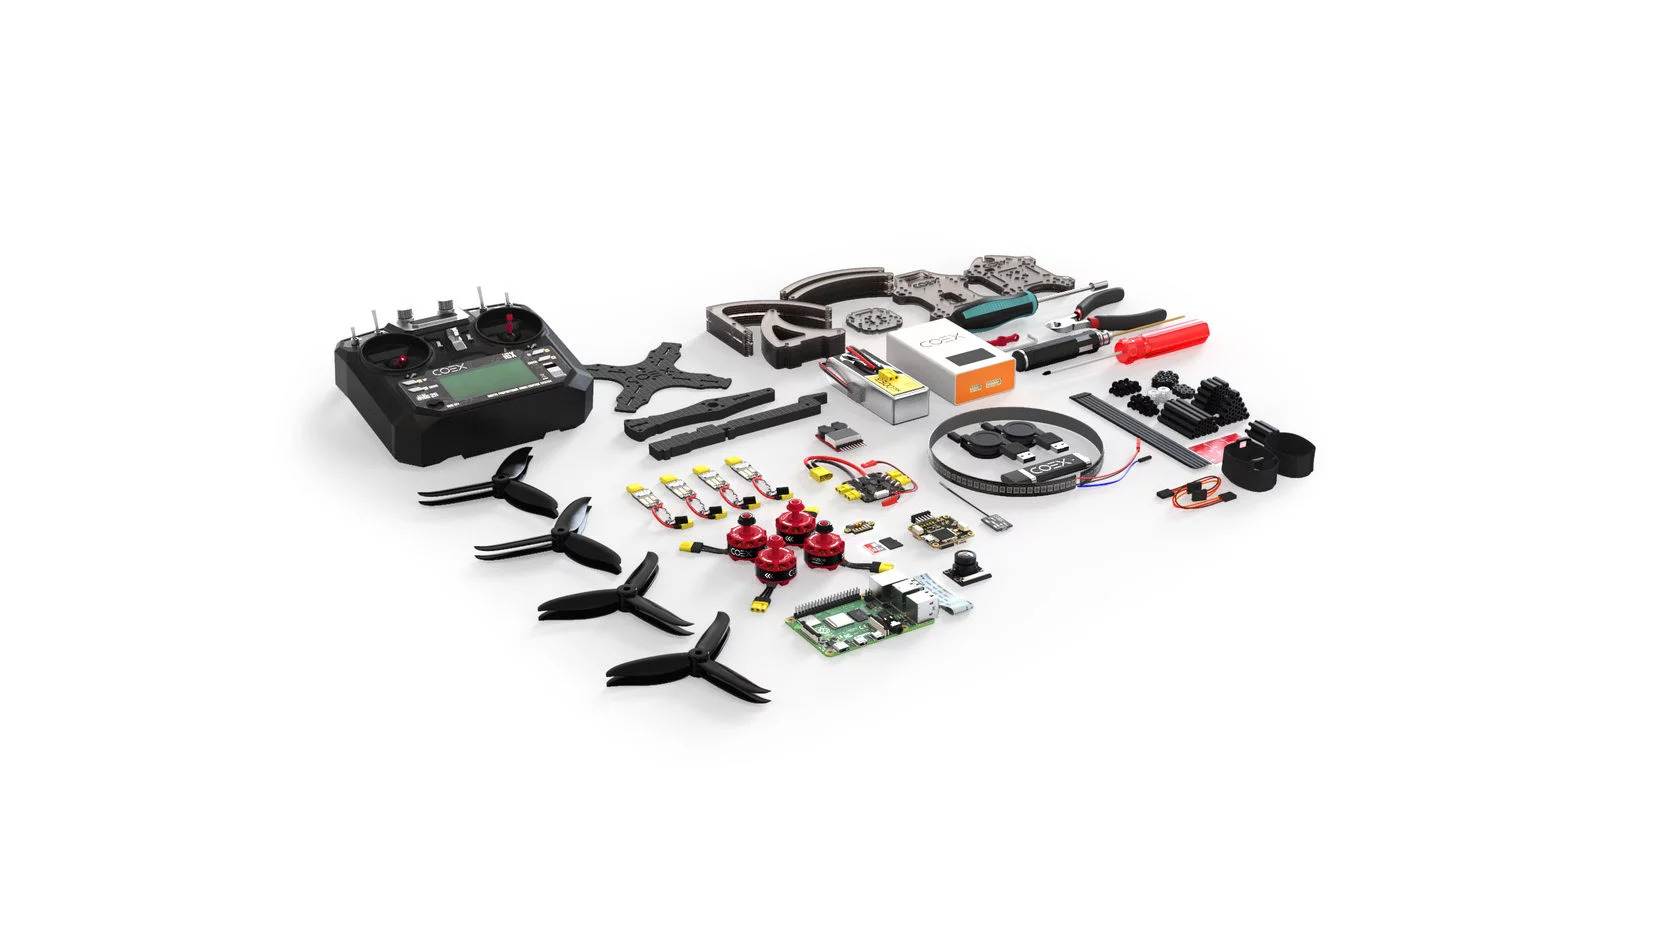
\includegraphics[width=10cm,keepaspectratio,angle=0]{images/coex_clover_kit.jpg}
    \caption[Bausatz Coex Clover Drohne]{\label{img coex_clover_kit} Bausatz Coex Clover Drohne \cite{img_coex_clover_kit}}
\end{figure}

Die Coex Clover Drohne soll laut Herstellerinformationen bis zu 15 Minuten am Stück fliegen können und in dieser Zeit eine Maximalhöhe von 500 Metern bei einer Höchstgeschwindigkeit von bis zu 72 km/h erreichen können \cite[vgl.][]{coex_clover}.\\

Zu den Hauptbestandteilen der Drohne zählen zum einen ein Raspberry Pi 4 sowie der Flightcontroller Coex Pix. Diese bilden die Grundlage zur Programmierung und Steuerung der Coex Clover Drohne und ermöglichen es zudem die Drohne über drahtlos per WLAN zu verbinden. \\
Die Drohne ist ein Quadrokopter und besitzt somit vier Motoren, welche einzelnd angesteuert werden können. Sie besitzt zudem eine Vielzahl verschiedener Sensoren, auf welche in Kapitel \ref{sensoren:section} genauer eingegangen wird. Zu diesen zählen unter anderem ein Gyroskop, Magnetometer sowie ein Laseranstandssensor und eine Kamera, die unten an der Drohne angebracht sind.
Zum Schutz befindet sich zudem außen einen Rahmen.
Bei der Drohne war zudem ein 2300 mAh großer Akku dabei, der für vom Hersteller angegebene Flugdauer sorgen soll.
Im Folgenden wird nun auf die wichtigsten Bestandteile der Coex Clover Drohne noch einmal genauer eingegangen:

\subsection{Raspberry Pi 4} \label{raspberry_pi:subsection}

\begin{figure}[htpb]
    \centering
    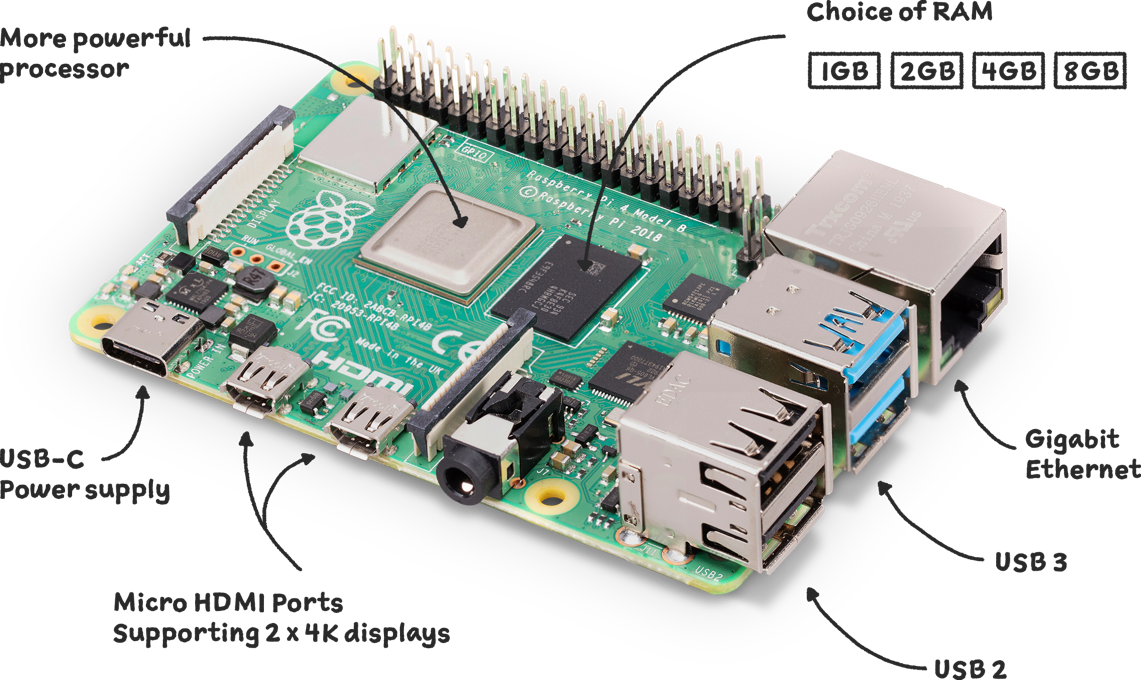
\includegraphics[width=10cm,keepaspectratio,angle=0]{images/raspberry-pi-4-labelled.png}
    \caption[Raspberry Pi 4]{\label{img raspberry_pi} Raspberry Pi 4 \cite{img_raspberry_pi}}
\end{figure}

Die Coex Clover Drohne enthält einen Raspberry Pi 4 Model B mit 1 GB Arbeitsspeicher.

\subsection{Coex Pix} \label{coex_pix:subsection}




\section{3D-Modelle} \label{3d-modelle:section}

    \subsection{3D-Scanning} \label{3d-scanning:subsection}

\section{Positionsbestimmung} \label{positionsbestimmung:section}

    \subsection{Spatial Mapping} \label{spatial_mapping:subsection}

    \subsection{Inertielle Positionsbestimmung} \label{inertielle_positionsbestimmung:subsection}

\section{Regelsysteme} \label{regelsysteme:section}

    \subsection{PID-Regler} \label{pid_regler:subsection}

    \subsection{Extended Kalman Filter 2}
    Der \ac{EKF}2-Algorithmus, der in der Drohnensteuerung verwendet wird, ist eine Erweiterung des klassischen erweiterten Kalman-Filters, die speziell auf die Bedürfnisse der Drohnensteuerung zugeschnitten ist. Der EKF2 ist ein geschätzter Zustandsregler, der die aktuellen Zustände (z.B. Position, Geschwindigkeit, Orientierung) einer Drohne schätzt, basierend auf Messungen von Sensoren (z.B. GPS, IMU, Magnetometer).

Im Gegensatz zum klassischen EKF verwendet der EKF2 eine modifizierte Version der Kalman-Filter-Formeln, um den Einfluss von Sensorrauschen und Messfehlern besser zu berücksichtigen. Insbesondere verwendet der EKF2 eine sogenannte "Innovation Covariance Matrix", die die Varianz der Messfehler repräsentiert und in die Filtergleichungen eingebaut wird. Diese Innovation Covariance Matrix wird iterativ während des Betriebs des Filters aktualisiert, um den Sensorrauschen und Messfehlern besser gerecht zu werden.

Darüber hinaus verwendet der EKF2 eine modifizierte Version der State Transition Matrix, die die Nichtlinearitäten des Systems besser modellieren kann. Diese modifizierte Matrix wird ebenfalls iterativ während des Filterbetriebs aktualisiert, um den Änderungen im Systemverhalten besser gerecht zu werden.

In der Drohnensteuerung wird der EKF2-Algorithmus verwendet, um die aktuellen Zustände der Drohne (z.B. Position, Geschwindigkeit, Orientierung) in Echtzeit zu schätzen. Diese Schätzungen werden dann verwendet, um die Steuerbefehle der Drohne zu generieren, um sie auf Kurs zu halten und sicher zu navigieren.

\section{Simulationstechnik} \label{simulationstechnik:section}

\section{Problembehebung} \label{problembehebung:section}
